%%%%%%%%%%%%%%%%%%%%%%%%%%%%%%%%%%%%%%%%%
% Masters/Doctoral Thesis 
% LaTeX Template
% Version 2.1 (2/9/15)
%
% This template has been downloaded from:
% http://www.LaTeXTemplates.com
%
% Version 2.0 major modifications by:
% Vel (vel@latextemplates.com)
%
% Original authors:
% Steven Gunn  (http://users.ecs.soton.ac.uk/srg/softwaretools/document/templates/)
% Sunil Patel (http://www.sunilpatel.co.uk/thesis-template/)
%
% License:
% CC BY-NC-SA 3.0 (http://creativecommons.org/licenses/by-nc-sa/3.0/)
%
%%%%%%%%%%%%%%%%%%%%%%%%%%%%%%%%%%%%%%%%%

%----------------------------------------------------------------------------------------
%	PACKAGES AND OTHER DOCUMENT CONFIGURATIONS
%----------------------------------------------------------------------------------------

\documentclass[
11pt, % The default document font size, options: 10pt, 11pt, 12pt
%oneside, % Two side (alternating margins) for binding by default, uncomment to switch to one side
ngerman, % ngerman for German
onehalfspacing, % Single line spacing, alternatives: onehalfspacing or doublespacing
%draft, % Uncomment to enable draft mode (no pictures, no links, overfull hboxes indicated)
%nolistspacing, % If the document is onehalfspacing or doublespacing, uncomment this to set spacing in lists to single
%liststotoc, % Uncomment to add the list of figures/tables/etc to the table of contents
%toctotoc, % Uncomment to add the main table of contents to the table of contents
%parskip, % Uncomment to add space between paragraphs
]{MastersDoctoralThesis} % The class file specifying the document structure

\usepackage[utf8]{inputenc} % Required for inputting international characters
\usepackage[T1]{fontenc} % Output font encoding for international characters

\usepackage{palatino} % Use the Palatino font by default

\usepackage[backend=bibtex,style=authoryear,natbib=true]{biblatex} % User the bibtex backend with the authoryear citation style (which resembles APA)

\addbibresource{references.bib} % The filename of the bibliography

\usepackage[autostyle=true]{csquotes} % Required to generate language-dependent quotes in the bibliography

%----------------------------------------------------------------------------------------
%	CODE STYLING
%-------------------------------------------------------------------------------

% Taken from Lena Herrmann at 
% http://lenaherrmann.net/2010/05/20/javascript-syntax-highlighting-in-the-latex-listings-package
\usepackage{listings}
\usepackage{color}

\definecolor{lightgray}{rgb}{.60, .60, .60}
\definecolor{darkgray}{rgb}{.40, .40, .40}

\lstdefinelanguage{JavaScript}{
  keywords={typeof, new, true, false, catch, function, return, null, catch, switch, var, if, in, while, do, else, case, break},
  keywordstyle=\color{black}\bfseries,
  ndkeywords={class, export, boolean, throw, implements, import, this},
  ndkeywordstyle=\color{black}\bfseries,
  identifierstyle=\color{black},
  sensitive=false,
  comment=[l]{//},
  morecomment=[s]{/*}{*/},
  commentstyle=\color{lightgray}\ttfamily,
  stringstyle=\color{darkgray}\ttfamily,
  morestring=[b]',
  morestring=[b]"
}

\lstset{
   language=JavaScript,
   extendedchars=true,
   basicstyle=\footnotesize\ttfamily,
   showstringspaces=false,
   showspaces=false,
   numbers=left,
   numberstyle=\footnotesize,
   numbersep=9pt,
   tabsize=2,
   breaklines=true,
   showtabs=false,
   captionpos=b
}


%----------------------------------------------------------------------------------------
%	THESIS INFORMATION
%----------------------------------------------------------------------------------------

\thesistitle{Objekt-relationale Mapper} % Your thesis title, this is used in the title and abstract, print it elsewhere with \ttitle
\supervisor{FOL Michael Rott} % Your supervisor's name, this is used in the title page, print it elsewhere with \supname
\examiner{} % Your examiner's name, this is not currently used anywhere in the template, print it elsewhere with \examname
\degree{Bachelor Informatik} % Your degree name, this is used in the title page and abstract, print it elsewhere with \degreename
\author{
	Florian \textsc{Duenow}\newline
	Sebastian \textsc{Pekarek}\newline
	Maximilian \textsc{May}\newline
	Florian \textsc{Kraus}
} % Your name, this is used in the title page and abstract, print it elsewhere with \authorname
\addresses{} % Your address, this is not currently used anywhere in the template, print it elsewhere with \addressname

\subject{Informatik} % Your subject area, this is not currently used anywhere in the template, print it elsewhere with \subjectname
\keywords{} % Keywords for your thesis, this is not currently used anywhere in the template, print it elsewhere with \keywordnames
\university{\href{http://www.fhws.de}{Hochschule für angewandte Wissenschaften Würzburg-Schweinfurt}} % Your university's name and URL, this is used in the title page and abstract, print it elsewhere with \univname
\faculty{\href{http://faculty.university.com}{Fakultät Informatik}} % Your faculty's name and URL, this is used in the title page and abstract, print it elsewhere with \facname

\hypersetup{pdftitle=\ttitle} % Set the PDF's title to your title
\hypersetup{pdfauthor=\authorname} % Set the PDF's author to your name
\hypersetup{pdfkeywords=\keywordnames} % Set the PDF's keywords to your keywords

\begin{document}

\frontmatter % Use roman page numbering style (i, ii, iii, iv...) for the pre-content pages
\pagenumbering{Roman}

\pagestyle{plain} % Default to the plain heading style until the thesis style is called for the body content

%----------------------------------------------------------------------------------------
%	TITLE PAGE
%----------------------------------------------------------------------------------------

\begin{titlepage}
\begin{center}

\textsc{\LARGE \univname}\\[1.5cm] % University name
\textsc{\Large Datenbanken II}\\[0.5cm] % Thesis type

\HRule \\[0.4cm] % Horizontal line
{\huge \bfseries \ttitle}\\[0.4cm] % Thesis title
\HRule \\[1.5cm] % Horizontal line
 
\begin{minipage}{0.4\textwidth}
\begin{flushleft} \large
\emph{Authoren:}\\
\authorname % Author name - remove the \href bracket to remove the link
\end{flushleft}
\end{minipage}
\begin{minipage}{0.4\textwidth}
\begin{flushright} \large
\emph{Dozent:} \\
\supname % Supervisor name - remove the \href bracket to remove the link  
\end{flushright}
\end{minipage}\\[3cm]

{\large \today}\\[4cm] % Date
%\includegraphics{Logo} % University/department logo - uncomment to place it
 
\vfill
\end{center}
\end{titlepage}

%----------------------------------------------------------------------------------------
%	LIST OF CONTENTS/FIGURES/TABLES PAGES
%----------------------------------------------------------------------------------------

\tableofcontents % Prints the main table of contents

%----------------------------------------------------------------------------------------
%	ABBREVIATIONS
%----------------------------------------------------------------------------------------

%\begin{abbreviations}{ll} % Include a list of abbreviations (a table of two columns)

%\textbf{LAH} & \textbf{L}ist \textbf{A}bbreviations \textbf{H}ere\\
%\textbf{WSF} & \textbf{W}hat (it) \textbf{S}tands \textbf{F}or\\

%\end{abbreviations}

%----------------------------------------------------------------------------------------
%	THESIS CONTENT - CHAPTERS
%----------------------------------------------------------------------------------------
\mainmatter % Begin numeric (1,2,3...) page numbering

\pagestyle{thesis} % Return the page headers back to the "thesis" style
% Include the chapters of the thesis as separate files from the Chapters folder
% Uncomment the lines as you write the chapters

% Chapter 1

\chapter{Einleitung} % Main chapter title

\label{Chapter1} % For referencing the chapter elsewhere, use \ref{Chapter1} 

%----------------------------------------------------------------------------------------

% Define some commands to keep the formatting separated from the content 
\newcommand{\keyword}[1]{\textbf{#1}}
\newcommand{\tabhead}[1]{\textbf{#1}}
\newcommand{\code}[1]{\texttt{#1}}
\newcommand{\file}[1]{\texttt{\bfseries#1}}
\newcommand{\option}[1]{\texttt{\itshape#1}}

%----------------------------------------------------------------------------------------

…

\section{Hintergrund und Problemstellung}

…

\section{Lösungsansätze}

…

\subsection{Objektorientierte Datenbanken}

…

\subsection{Objekt-relationale Datenbanken}

…

\subsection{Programmierspache um relationale Funktionalitäten erweitern}

…

\subsection{Objekt-relationale Mapper}

…

% Chapter 2

\chapter{Abstraktes Beispiel} % Main chapter title

\label{Chapter2} % For referencing the chapter elsewhere, use \ref{Chapter2} 

Objektorientierte Programmiersprachen speichern Attribute und Methoden in Objekten, wehrend relationale Datenbanken ihre Daten in flachen Tabellen speichert. Aufgrund dieser beiden unterschiedlichen Konzepte entsteht ein Konzeptioneller Wiederspruch auch als object-relational impedance missmatch bekannt.

\begin{figure}[h]
\begin{center}
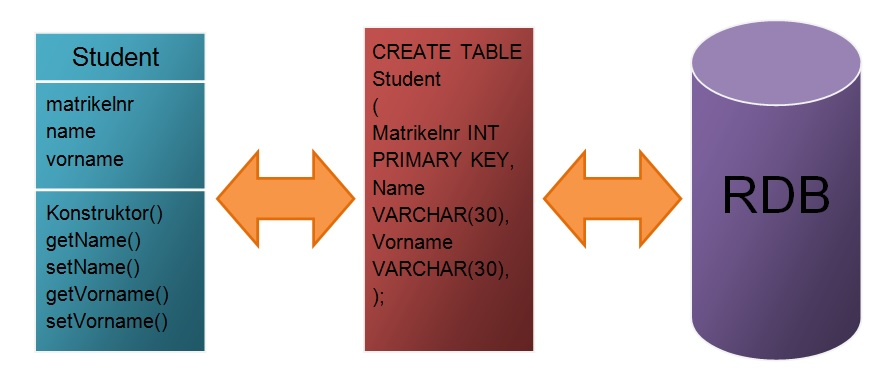
\includegraphics[width=1.0\textwidth]{ORM_Bild1.jpg}
\end{center}
\end{figure}

\newpage
Um diesen Widerspruch weit möglichst aufzulösen haben sich ORMs etabliert diese bieten den Vorteil das keine SQL Statements mehr im Programmcode notwendig sind, da diese vom ORM Framework automatisch generiert werden. Ein weiterer Vorteil ist das die Programmiersprache selbst nicht erweitert werden muss, da die Implementierung normalerweise über Klassenbibliotheken abgewickelt wird.

\begin{figure}[h]
\begin{center}
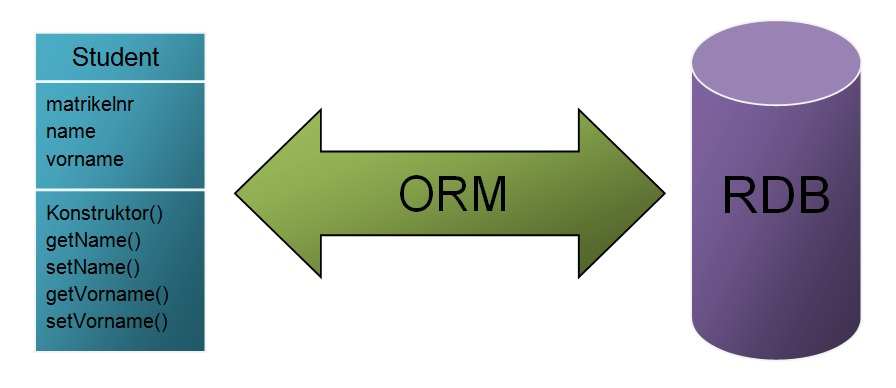
\includegraphics[width=1.0\textwidth]{ORM_Bild2.jpg}
\end{center}
\end{figure}
 
% Chapter 3

\chapter{Konkrete Beispiele} % Main chapter title

\label{Chapter3} % For referencing the chapter elsewhere, use \ref{Chapter3} 

\section{JavaScript – Sequelize}


Sequelize ist ein objektrelationaler Mapper, der im Rahmen einer Masterarbeit von Sascha Depold entwickelt wurde. Als Laufzeitumgebung wurde Node.js gewählt, in der die aus dem Browser bekannte Programmiersprache JavaScript interpretiert wird. Durch asynchrone Patterns in der Sprache, z.B. Callbacks oder Promises, ist sie sehr gut für die Abarbeitung paralleler Prozesse geeignet.

\subsection{Grundlagen}

\paragraph{Relationale Zugriffsschicht} \hspace{0pt} \\
Sequelize bedient sich des Entwurfsmusters des Data Access Object (DAO). Dies beschreibt die Nutzung spezieller Klassen zum Zugriff auf Datenquellen. Die Klassen definieren dabei die zum einen die Schnittstellen zwischen den Daten und der Geschäftslogik. So kann sichergestellt werden, dass die Schnittstellen selbst beim Austausch des Datenbanksystems (also der Datenquelle) existent und konsistent bleiben (\cite[S. 8]{Depo1}). Aufgabe des DAO ist es unter anderem, die Datenquelle (Datenbank) abzufragen, die Ergebnisse entgegenzunehmen und sie in ein entsprechendes Datenobjekt (Data Transfer Object, DTO) zu konvertieren.

\begin{lstlisting}[caption=Relationale Zugriffsschicht]
class StudentDAO
  def self.all
    query = "SELECT * FROM students"
    return SQLConnector.execurte(query)
  end
  
  def self.update(attributes, id)
    query = "UPDATE students (" + attributes.keys.join(",") + ") VALUES ("
    query += attributes.values.join(",") + ") WHERE id=" + id
    return SQLConnector.execute(query)
  end
end

class StudentController
  def index
    @students = StudentDAO.all
  end
end
\end{lstlisting}


\paragraph{Objektrelationale Zugriffsschicht} \hspace{0pt} \\

Diese Schicht ermöglicht das Arbeiten mit den nun nicht mehr repräsentativen Geschäftsobjekten. Dadurch wird die Manipulation dieser Objekte ermöglicht. Außerdem können nur weitere Features wie z.B. Assoziationen oder Berechtigungen implementiert werden. Auch das Löschen von Datensätzen ist nun möglich.

\begin{lstlisting}[caption=Objektrelationale Zugriffsschicht]
class StudentDAO
  def self.all
    results = SQLConnector.execute("SELECT * FROM students")
    users = results.map{ |hash| return new UserDO(hash) }
    return users;
  end
  
  def self.find(id)
    result = SQLConnector.execute("SELECT * FROM students WHERE id=" + id)
    return new UserDTO(result)
  end
end

class StudentDTO
  def update(attributes)
    query = "UPDATE students (" + attributes.keys.join(",") + ") VALUES ("
    query += attributes.values.join(",") + ") WHERE id=" + self.id
    return SQLConnector.execute(query)
  end
end

class StudentController
  def index
    @students = StudentDAO.all
  end
end
\end{lstlisting}

Um doppelten Code zu vermeiden, sollte die Architektur jedoch leicht abgeändert werden. So wird die DAO- bzw. Datenobjekt-Logik in eine Oberklasse ausgelagert und entsprechende Vererbung eingeführt (\cite[S. 11]{Depo1}).


\subsection{Architektur}

\paragraph{Sequelize} \hspace{0pt} \\
Die Klasse Sequelize ist der zentrale Einstiegspunkt des Mappers. Sie ermöglicht das Definieren von DAO-Factories und Konfiguration.

\paragraph{DAOFactory (Model)} \hspace{0pt} \\
Klasse, die die Struktur einer Datenbanktabelle widerspiegelt. Dafür müssen Instanzen den jeweiligen Tabellennamen und die Attribute enthalten. Die Klasse stellt Methoden bereit, um die Tabelle auszulesen oder eine DAO-Instanz zu erstellen.

\paragraph{DAO (Instance)} \hspace{0pt} \\
Instanzen der DAO-Klasse spiegeln einzelne Datenbankeinträge wieder. Sie werden u.A. durch den Aufruf der build()-oder create()-Method der DAOFactory erzeugt.


\subsection{Benutzung}

\paragraph{Klassendefinition} \hspace{0pt} \\

Sequelize verfolgt den Modell- und den Schemagetriebenen Ansatz zur Definition von Modellen. Dies hat zur Folge, dass alle Models vorher definiert werden müssen.

\begin{lstlisting}[caption=Klassendefinition (Sequelize)]
var Student = sequelize.define('student', {
  firstname: Sequelize.STRING(40)
  lastname: Sequelize.STRING(40)
});	
\end{lstlisting}

Die Spalten `id`, `created\_at` und `updated\_at` müssen nicht definiert werden, diese werden von Sequelize automatisch erzeugt.


\paragraph{Datensatz abfragen} \hspace{0pt} \\

Sequelize stellt in der Klasse DAOFactory mehrere Methoden bereit, mit denen sich Daten aus Tabellen auslesen lassen, z.B. `find()`, `findAll()` und `count()`. Über Optionen wie z.B. `where`, `limit` oder `offset` können die Suchen jeweils angepasst werden.

\begin{lstlisting}[caption=Datensatz abfragen (Sequelize)]
Student.find({
  where: {
    id: {
      $between: [12000, 14000],
      $notIn: [12900, 13000]
    },
    name: 'Meier'
  }
}).then(function(student) {
  console.log('Student: %j', student);
});	
\end{lstlisting}


\paragraph{Datensatz anlegen} \hspace{0pt} \\

Die Methoden `DAOFactory.build()` und `DAOFactory.create()` ermöglichen es, sowohl temporäre als auch persistente Datenbankeinträge zu erstellen. Mit `DAO.save()` wird der temporäre, ungespeicherte Eintrag in der Datenbank gespeichert.

\begin{lstlisting}[caption=Datensatz anlegen (Sequelize)]
// ungespeichertes Model erstellen
var student = Student.build({
  firstname: 'Max',
  lastname: 'Mustermann'
});

// Model speichern
student.save().then(function() {
  // Und alle so: Yeah!
});	
\end{lstlisting}


\paragraph{Datensatz modifizieren} \hspace{0pt} \\

Über die Methoden `save()` und `destroy()` der DAO-Klasse ist es jederzeit möglich, Objekte zu verändern oder zu löschen.

\begin{lstlisting}[caption=Datensatz ändern (Sequelize)]
	student.firstname = 'Moritz';
	student.save();
\end{lstlisting}

\begin{lstlisting}[caption=Datensatz löschen (Sequelize)]
	student.destroy();
\end{lstlisting}



\paragraph{Assoziationen} \hspace{0pt} \\

Nach dem definieren von Models ist es mit Sequelize möglich, Assoziationen zu definieren. Dabei sind 1:1-, 1:m- und n:m-Assoziationen möglich.

\begin{lstlisting}[caption=Datensatz anlegen (Sequelize)]
	var Student = sequelize.define('student', {/* Definition */}),
    	StudyCourse = sequelize.define('studyCourse', {/* Definition */});
	
	StudyCourse.belongsTo(StudyCourse);
\end{lstlisting}

Diese Definition würde nun zur Tabelle `student` den Foreign-Key `studyCourseId` hinzufügen, um die 1:m-Beziehung abbilden zu können.






\section{Python – SQLAlchemy}

SQLAlchemy\footnote{\href{http://www.sqlalchemy.org/}{http://www.sqlalchemy.org/}} ist ein Objekt-relationaler Mapper für die Programmiersprache Python. Das Framework wurde im Februar 2006 von Michael Bayer unter der MIT Lizenz – als Open Source – veröffentlicht. Seitdem gewann es an sehr großer Beliebtheit, vor allem in der Open Source Welt, aber auch bei großen und bekannten Firmen\footnote{\href{http://www.sqlalchemy.org/organizations.html}{http://www.sqlalchemy.org/organizations.html}} wie Dropbox, Hulu oder Uber.

\subsection{Allgemein}

\paragraph{Philosophie} \hspace{0pt} \\
SQL databases behave less like object collections the more size and performance start to matter; object collections behave less like tables and rows the more abstraction starts to matter. SQLAlchemy aims to accommodate both of these principles.

\paragraph{Unterstützte Datenbanken (Dialekte)} \hspace{0pt} \\
\begin{itemize}
	\item MySQL
	\item SQLite
	\item PostgreSQL
	\item Oracle
	\item Microsoft SQL Server
\end{itemize}

Es ist außerdem relativ einfach einen weiteren Dialekt in SQLAlchemy zu integrieren. SAP hat dies zum Beispiel für seine HANA-Datenbank realisiert\footnote{\href{https://github.com/SAP/sqlalchemy-hana}{https://github.com/SAP/sqlalchemy-hana}}.

\subsection{Komponenten}
SQLAlchemy besteht aus zwei alleinstehenden Komponenten: Dem Core und dem ORM.

\paragraph{Core} \hspace{0pt} \\
Der Core ist ein Abstraktionslayer für verschiedene Datenbank-API-Implementierungen, welcher es erlaubt SQL-Abfragen über eine allgemeine Syntax in Python zu schreiben ("`SQL Expression Language"').

\begin{lstlisting}[language=Python]
select([Student.id, Student.martrikelnr])
.where(Student.name == 'Peter')
.order_by(Student.name)
\end{lstlisting}

\hspace{0pt}

\noindent
Außerdem bietet er die Möglichkeit jeden Datentyp von Python auf einen SQL-Datentypen zu "`mappen"'. Ein Beispiel hierfür wäre der Datentyp \textit{Decimal} in Python; dieser wird auf \textit{NUMERIC} in PostgreSQL und \textit{DECIMAL} auf SQL Server konvertiert. Dies hat den Vorteil, dass man mit dem nativen Datentypen der Programmiersprache Python arbeiten kann und sich nicht explizit darum kümmmern muss, welcher Datentyp in der Datenbank hierfür verwendet wird.

\paragraph{ORM} \hspace{0pt} \\
Der ORM (Objekt-relationale Mapper) ermöglicht das klassische „Mappen“ von Datenbank-Tabellen auf Objekte. Er erlaubt nicht nur das Mapping auf einzelne Tabellen, sondern ermöglicht auch Objektorientierte Paradigmen wie Vererbung. Referenzierungen über Fremdschlüssel sind ebenfalls möglich.

\begin{lstlisting}[language=Python]
class Studiengang(Model):
    __tablename__ = 'studiengaenge'

    id = Column(
        Integer(),
        primary_key=True
    )

    name = Column(
        Unicode(),
        nullable=False,
        unique=True
    )


class Student(Model):
    __tablename__ = 'studenten'

    id = Column(
        Integer(),
        primary_key=True
    )

    name = Column(
        Unicode(255),
        nullable=False
    )

    studiengang_id = Column(
        Integer(),
        ForeignKey('studiengaenge.id'),
        nullable=False
    )
    studiengang = relationship(
        Studiengang,
        lazy='joined',
        backref='studenten'
    )
\end{lstlisting}


Anhand dieser Klassendefinitionen können nun zwei Tabellen angelegt werden. SQLAlchemy kann anhand der o. g. Notationen die nötigen SQL-Statements (CREATE TABLE …) erzeugen.

\hspace{1.0pt}

\noindent
Das Anlegen eines neuen Datensatzes sieht nun folgendermaßen aus:

\begin{lstlisting}[language=Python]
studiengang = Studiengang()
studiengang.name = 'Informatik'

student = Student()
student.name = 'Peter'
student.studiengang = studiengang

session.add(student)
session.commit()
\end{lstlisting}

Die INSERT-Statements werden nun mithilfe der "`Unit of Work"'\footnote{Vgl. Essential SQLAlchemy, S. 94f} in der richtigen Reihenfolge ausgeführt, sowie die Fremdschlüsselreferenz von \textit{student.studiengang\_id} automatisch aufgelöst.

\subsection{Unit of Work}

Die Unit of Work ist ein integraler Bestandteil von SQLAlchemy’s ORM-Erweiterung. Diese folgt dem "`Unit of Work"'-Pattern von Martin Fowler\footnote{\href{http://martinfowler.com/eaaCatalog/unitOfWork.html}{http://martinfowler.com/eaaCatalog/unitOfWork.html}}, welches bspw. auch von Hibernate (Java’s populärster ORM) genutzt wird.

Änderungen an Objekte werden beim Unit of Work-System nicht direkt in die Datenbank geschrieben, sondern gesammelt in einer Transaktion abgeschickt. Hierfür wird eine topologische Sortierung nach Abhängigkeiten durchgeführt, um z. B. Fremdschüsselreferenzen (siehe o. g. Beispiel) aufzulösen. Diese System hat außerdem den Vorteil, dass redundante Anfragen gebündelt und Deadlocks vermieden werden können.

\section{Java – Hibernate}

Hibernate ist ein ORM-Framework für Java, dessen Hauptaufgabe die objektrelationale Abbildung ist. Dies ermöglicht Klassen, Objekte und Attribute in relationalen Datenbaken zu speichern und auszulesen, dabei gilt:

\begin{itemize}
	\item Jede Klasse entspricht eine Tabelle
	\item Jedes Objekt entspricht einem Datensatz
	\item Jedes Attribut entspricht einer Spalte.
\end{itemize}
(\cite[S. 280]{Piep1})

\subsection{Grundlagen}

Um ein Tabelle aus einer Java Klasse zu erstellen muss das SQL Statement aus einzelnen Attributen des Java Objekts generiert werden. Dabei liegt aber ein Konzeptioneller Wiederspruch zwischen der Objektorientierten Struktur und der flachen Tabellenstruktur vor. Auch Objektrelationaler Bruch genannt. Hibernate fungiert hier als Verbindungsglied zwischen Java und der Relationalen Datenbank. Indem es automatisch SQL Statements aus Java Objekten abstrahiert.


\subsection{Hibernate Konventionen}

Um ein Java-Objekt mittels Hibernate in einer relationalen Datenbank persistent zu verwalten, muss die Klasse des Objektes einige grundlegende Notationen befolgen. Zunächst muss die Klasse mit der Annotation @Entity versehen werden damit sie in Datenbank gemappt werden kann. „Die Annotation @Entity macht aus einer „normalen“ Klasse eine Klasse, deren Instanzen mit einer JPA-Implementierung persistent gemacht werden können.“(\cite[S. 32]{MW1}) Welche Spalte der Primärschlüssel sein soll muss angegeben werden. Dies geschieht mit der Annotation @Id. Die Annotation des Primärschlüssels kann bei der Instanzvariablen oder bei Getter/ Setter-Paar stehen und definiert damit dem Zugriff der JPA-Implementierung auf das Property. Im unteren Beispiel mit Attribut Matrikelnummer geschehen. (\cite[S. 32]{MW1})

Die Attribute sind als privat deklariert, daher werden entsprechend der Java-Konventionen set/get-Methoden für jedes Attribut definiert, die auch von Hibernate so erwartet werden.(\cite[S. 454]{SSH1}) Zu beachten ist das Hibernate einen default Konstruktor erwartet, also einen Parameterfreien Konstruktor, welcher zwar bei keiner Angebe eines Konstruktors automatisch von Java mit initialisiert wird, aber nochmal explizit angegeben werden muss wenn ein weiterer Konstruktor vorhanden ist.

\hspace{0pt}
\begin{lstlisting}[language=Java]
@Entity
public class Student {
	
	@Id
	private int matrikelnummer;
	private String name;
	private String vorname;
	private String email;
	private String studiengang;
	
	public int getMatrikelnummer() {
		return matrikelnummer;
	}

	public void setMatrikelnummer(int matrikelnummer) {
		this.matrikelnummer = matrikelnummer;
	}

	public String getName() {
		return name;
	}

	public void setName(String name) {
		this.name = name;
	}

	// ...
	
	public Student() {};
	
	public Student(int matrikelnummer, String name, String vorname, String email, String studiengang) {
		this.matrikelnummer = matrikelnummer;
		this.name = name;
		this.vorname = vorname;
		this.email = email;
		this.studiengang = studiengang;
	}
}

\end{lstlisting}

\subsection{Data Access Objekt Pattern}

Über das Entwurfsmuster des DAO trennen wir die Programmlogik  von den technischen Details der Erstellung eines Tabels. Zudem verwenden wir das DAO Pattern zum Speichern, Auslesen etc. unseres Objektes.

\paragraph{Sitzung und Transaktion} \hspace{0pt} \\
Zunächst müssen wir die Aktuelle Session öffnen und die Transaktion beginnen. Dies erreichen wir über die Methoden getCurrentSession und beginTransaction welche ich im unteren Beispiel in der Methode openSessionAndTransaction aufrufe. Als Rückgebewert bekommen wir die aktuelle Sitzung. Beim Schließen der Sitzung ist darauf zu achten das Transaktion zunächst Kommittet wird bevor die Sitzung beendet wird (siehe closeSessionAndTransaction).

\paragraph{Zugriff über die DAO} \hspace{0pt} \\
Über das DAO können wir auf verschiedene weisen auf Daten unseres Objektes zugreifen. So können wir nicht nur Objekte speichern oder löschen sondern auch Datensätze ändern oder nach ihnen suchen.

\hspace{0pt}
\begin{lstlisting}[language=Java]
public class StudentDAO {
	
	private Session session;
	private Transaction transaction;
	
	public StudentDAO() {} 

	public Session openSessionAndTransaction() {
		session = HibernateUtil.getSessionFactory().getCurrentSession();
		transaction = session.beginTransaction();
		return session;
	}
	
	public void closeSessionAndTransaction() {
		transaction.commit();
		session.close();
	}
	
	public Session getSession(){
		return session;
	}
	
	public void save(Student s) {
		getSession().save(s);
	}
	
	public void update(Student s) {
		getSession().update(s);
	}
	
	public Student find(int matrikelnummer) {
		Student s = (Student) getSession().get(Student.class, 
				matrikelnummer);
		return s;
	}
	
	public void delete(Student s) {
		getSession().delete(s);
	}

}

\end{lstlisting}


% Chapter 4

\chapter{Demo} % Main chapter title

\label{Chapter4} % For referencing the chapter elsewhere, use \ref{Chapter4} 

…
 

%----------------------------------------------------------------------------------------
%	THESIS CONTENT - APPENDICES
%----------------------------------------------------------------------------------------

\appendix % Cue to tell LaTeX that the following "chapters" are Appendices

% Include the appendices of the thesis as separate files from the Appendices folder
% Uncomment the lines as you write the Appendices

%% Appendix A

\chapter{Anhang} % Main appendix title

\label{AppendixA} % For referencing this appendix elsewhere, use \ref{AppendixA}

…

%\input{Appendices/AppendixB}
%\input{Appendices/AppendixC}

%----------------------------------------------------------------------------------------
%	BIBLIOGRAPHY
%----------------------------------------------------------------------------------------

\printbibliography[heading=bibintoc]

%----------------------------------------------------------------------------------------

\end{document}  
